\documentclass[10pt,letterpaper]{article}

% Packages
\usepackage[margin=0.5in]{geometry}
\usepackage[utf8]{inputenc}
\usepackage[T1]{fontenc}
\usepackage{helvet}
\renewcommand{\familydefault}{\sfdefault}
\usepackage{xcolor}
\usepackage{tcolorbox}
\usepackage{array}
\usepackage{tabularx}
\usepackage{booktabs}
\usepackage{enumitem}
\usepackage{titlesec}
\usepackage{fancyhdr}
\usepackage{multicol}
\usepackage{graphicx}
\usepackage{tikz}
\usetikzlibrary{shapes,arrows,positioning}

% Color definitions
\definecolor{headerblue}{RGB}{0,102,204}
\definecolor{stronggreen}{RGB}{0,153,76}
\definecolor{conditionalyellow}{RGB}{255,193,7}
\definecolor{researchblue}{RGB}{33,150,243}
\definecolor{warningred}{RGB}{204,0,0}
\definecolor{highlightgray}{RGB}{240,240,240}

% Section formatting - compact
\titleformat{\section}{\normalfont\fontsize{11}{12}\bfseries\color{headerblue}}{\thesection}{0.5em}{}
\titlespacing*{\section}{0pt}{4pt}{2pt}

\titleformat{\subsection}{\normalfont\fontsize{10}{11}\bfseries}{\thesubsection}{0.5em}{}
\titlespacing*{\subsection}{0pt}{3pt}{1pt}

% List formatting - ultra compact
\setlist[itemize]{leftmargin=*,itemsep=0pt,parsep=0pt,topsep=1pt}
\setlist[enumerate]{leftmargin=*,itemsep=0pt,parsep=0pt,topsep=1pt}

% Remove paragraph indentation
\setlength{\parindent}{0pt}
\setlength{\parskip}{2pt}

% Header/footer
\pagestyle{fancy}
\fancyhf{}
\fancyhead[L]{\footnotesize \textbf{Treatment Recommendations: [CONDITION]}}
\fancyhead[R]{\footnotesize Page \thepage}
\renewcommand{\headrulewidth}{0.5pt}
\fancyfoot[C]{\footnotesize Evidence-Based Clinical Guideline - For Professional Use Only}

\begin{document}

% Title block
\begin{center}
{\fontsize{14}{16}\selectfont\bfseries\color{headerblue} EVIDENCE-BASED TREATMENT RECOMMENDATIONS}\\[2pt]
{\fontsize{12}{14}\selectfont\bfseries [Disease/Condition - e.g., HER2+ Metastatic Breast Cancer]}\\[2pt]
{\fontsize{10}{12}\selectfont [Institution/Organization]}\\[1pt]
{\fontsize{9}{11}\selectfont Version X.X | Effective Date: [Date] | Next Review: [Date]}
\end{center}

\vspace{4pt}

% Recommendation Strength Legend
\begin{tcolorbox}[colback=highlightgray,colframe=black,title=\textbf{Recommendation Strength Key},fonttitle=\bfseries\small,coltitle=black]
{\small
\begin{itemize}
\item \colorbox{stronggreen!30}{\textbf{STRONG (Grade 1)}} - Benefits clearly outweigh risks; most patients should receive intervention
\item \colorbox{conditionalyellow!30}{\textbf{CONDITIONAL (Grade 2)}} - Trade-offs exist; shared decision-making essential
\item \colorbox{researchblue!30}{\textbf{RESEARCH (Grade R)}} - Insufficient evidence; clinical trial enrollment preferred
\end{itemize}

\textbf{Evidence Quality}: \textbf{A} = High (RCTs), \textbf{B} = Moderate (RCTs with limitations), \textbf{C} = Low (observational), \textbf{D} = Very low (expert opinion)
}
\end{tcolorbox}

\vspace{2pt}

\section{Clinical Context}

\subsection{Disease Overview}

[Brief description of disease state, epidemiology, natural history]

\subsection{Patient Population}

\textbf{Target Population}:
\begin{itemize}
\item [Demographic characteristics - e.g., Adults $\geq$18 years]
\item [Disease stage/severity - e.g., Metastatic disease, Stage IV]
\item [Biomarker status - e.g., HER2-positive (IHC 3+ or FISH+)]
\item [Performance status - e.g., ECOG 0-2]
\item [Line of therapy - e.g., First-line, previously untreated]
\end{itemize}

\textbf{Exclusions}:
\begin{itemize}
\item [Contraindications to recommended therapies]
\item [Comorbidities affecting eligibility]
\end{itemize}

\section{Evidence Review}

\subsection{Key Clinical Trials}

\textbf{[Trial Name 1]} (Author, Journal Year):
\begin{itemize}
\item \textbf{Design}: Phase 3 RCT, n=XXX, [Treatment A] vs [Treatment B]
\item \textbf{Population}: [Key eligibility criteria]
\item \textbf{Primary Endpoint}: [Outcome] - XX vs XX months (HR X.XX, 95\% CI X.XX-X.XX, p<X.XXX)
\item \textbf{Secondary Endpoints}: [Additional outcomes]
\item \textbf{Safety}: Grade 3-4 AEs XX\% vs XX\%
\item \textbf{Quality}: \textbf{High} (low risk of bias, adequate power, intention-to-treat analysis)
\end{itemize}

\textbf{[Trial Name 2]} (Author, Journal Year):
\begin{itemize}
\item \textbf{Design}: Phase 3 RCT, n=XXX, [Treatment C] vs [Standard of care]
\item \textbf{Primary Endpoint}: [Outcome and results]
\item \textbf{Quality}: \textbf{Moderate} (some limitations)
\end{itemize}

\subsection{Guideline Concordance}

\begin{table}[H]
\centering
\small
\begin{tabular}{lll}
\toprule
\textbf{Guideline} & \textbf{Recommendation} & \textbf{Evidence Level} \\
\midrule
NCCN vX.XXXX & [Specific recommendation] & Category 1 (preferred) \\
ASCO Year & [Recommendation] & Strong, Evidence A \\
ESMO Year & [Recommendation] & Grade I, A \\
\bottomrule
\end{tabular}
\caption{Major guideline recommendations}
\end{table}

\section{Treatment Options}

\subsection{First-Line Therapy}

\begin{tcolorbox}[enhanced,colback=stronggreen!10,colframe=stronggreen,
title={\textbf{Option 1: [Regimen Name]} \hfill \colorbox{white}{\textbf{STRONG (1A)}}},
fonttitle=\bfseries\small,coltitle=black]
{\small
\textbf{Regimen}:
\begin{itemize}
\item [Drug A]: XX mg [IV/PO] [schedule]
\item [Drug B]: XX mg [IV/PO] [schedule]
\item Cycle length: XX days
\item Duration: Until progression or unacceptable toxicity
\end{itemize}

\textbf{Evidence Basis}:
\begin{itemize}
\item Primary study: [Trial name], n=XXX
\item Primary outcome: [Endpoint] XX vs XX months (HR X.XX, p<X.XXX)
\item ORR: XX\% vs XX\% (control)
\end{itemize}

\textbf{Indications}:
\begin{itemize}
\item [Biomarker-defined population or all patients]
\item [Performance status requirement]
\item [Organ function requirements]
\end{itemize}

\textbf{Key Toxicities}:
\begin{itemize}
\item Grade 3-4 AEs: XX\%
\item Common: [List 3-5 most common AEs with incidence]
\item Serious: [SAEs, discontinuation rate]
\item Management: [Key mitigation strategies]
\end{itemize}

\textbf{Monitoring}:
\begin{itemize}
\item Labs: [Specific tests, frequency]
\item Imaging: Every [X weeks] (RECIST v1.1)
\item Clinical assessment: Every cycle
\end{itemize}

\textbf{Recommendation Strength}: \textbf{STRONG} - Benefits clearly outweigh risks\\
\textbf{Evidence Quality}: \textbf{HIGH} - Well-designed RCT with consistent results
}
\end{tcolorbox}

\vspace{3pt}

\begin{tcolorbox}[enhanced,colback=conditionalyellow!10,colframe=conditionalyellow,
title={\textbf{Option 2: [Alternative Regimen]} \hfill \colorbox{white}{\textbf{CONDITIONAL (2B)}}},
fonttitle=\bfseries\small,coltitle=black]
{\small
\textbf{Regimen}: [Dosing details]

\textbf{Evidence Basis}: [Moderate-quality evidence or specific population subset]

\textbf{Indications}: [When to consider this option - e.g., patient preference for oral therapy, specific contraindication to Option 1]

\textbf{Trade-offs}: 
\begin{itemize}
\item Advantages: [e.g., Oral administration, better tolerability]
\item Disadvantages: [e.g., Lower response rate, less survival benefit]
\end{itemize}

\textbf{Recommendation Strength}: \textbf{CONDITIONAL} - Patient values important in decision\\
\textbf{Evidence Quality}: \textbf{MODERATE} - Some limitations in evidence base
}
\end{tcolorbox}

\vspace{3pt}

\begin{tcolorbox}[enhanced,colback=researchblue!10,colframe=researchblue,
title={\textbf{Option 3: Clinical Trial} \hfill \colorbox{white}{\textbf{RESEARCH (R)}}},
fonttitle=\bfseries\small,coltitle=black]
{\small
\textbf{Recommendation}: Consider clinical trial enrollment for [specific scenario - e.g., biomarker-selected patients, refractory disease]

\textbf{Available Trials}: [List relevant trials if known, or state "ClinicalTrials.gov search"]

\textbf{Rationale}: [Why clinical trial appropriate - e.g., novel mechanism, unmet medical need, investigational biomarker]
}
\end{tcolorbox}

\subsection{Second-Line and Beyond}

\textbf{At Progression on First-Line Therapy}:

\begin{itemize}
\item \textbf{Biomarker Re-Testing}: [If applicable - e.g., liquid biopsy for resistance mutations]
\item \textbf{Second-Line Options}:
  \begin{itemize}
  \item Preferred: [Regimen] (Evidence level)
  \item Alternative: [Regimen] (Evidence level)
  \end{itemize}
\item \textbf{Third-Line Options}: [Subsequent therapy options]
\end{itemize}

\section{Special Populations}

\subsection{Elderly Patients ($\geq$70 years)}

\textbf{Considerations}:
\begin{itemize}
\item Geriatric assessment recommended (G8 screening tool)
\item Dose reductions: [Specific adjustments for frail patients]
\item Monitoring: More frequent assessments for toxicity
\end{itemize}

\textbf{Regimen Modifications}:
\begin{itemize}
\item [Reduced-intensity regimens if appropriate]
\item [Single-agent vs combination considerations]
\end{itemize}

\subsection{Renal Impairment}

\begin{table}[H]
\centering
\footnotesize
\begin{tabular}{lll}
\toprule
\textbf{eGFR (mL/min/1.73m²)} & \textbf{Category} & \textbf{Dose Adjustment} \\
\midrule
$\geq$60 & Normal/Mild & Standard dosing \\
30-59 & Moderate & [Specific adjustment - e.g., Reduce 25\%] \\
15-29 & Severe & [Specific adjustment - e.g., Reduce 50\% or avoid] \\
<15 or dialysis & ESRD & [Use with caution or contraindicated] \\
\bottomrule
\end{tabular}
\caption{Dose adjustments for renal impairment}
\end{table}

\subsection{Hepatic Impairment}

[Similar table for hepatic dose adjustments using Child-Pugh class or bilirubin/transaminases]

\section{Clinical Decision Algorithm}

% Simple flowchart example - can be expanded with more complex TikZ
\begin{center}
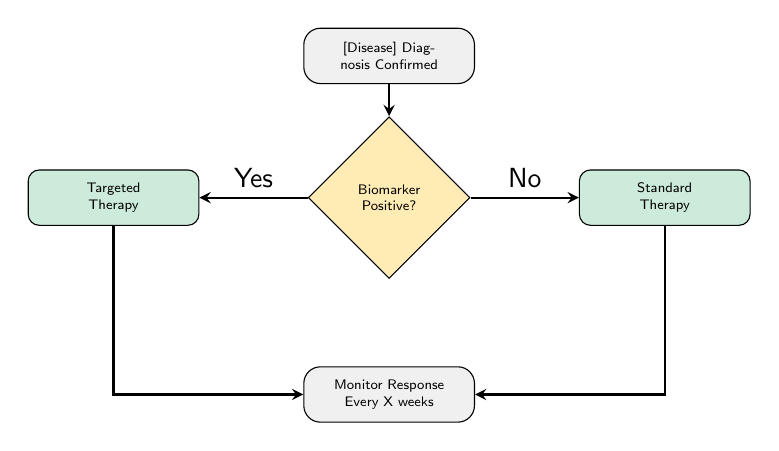
\begin{tikzpicture}[node distance=1.8cm, auto,
  decision/.style={diamond, draw, fill=conditionalyellow!30, text width=4.5em, text centered, inner sep=1pt, font=\tiny},
  process/.style={rectangle, draw, fill=stronggreen!20, text width=5.5em, text centered, rounded corners, minimum height=2em, font=\tiny},
  terminal/.style={rectangle, draw, fill=highlightgray, text width=5.5em, text centered, rounded corners=6pt, minimum height=2em, font=\tiny},
  alert/.style={rectangle, draw=warningred, line width=1pt, fill=warningred!10, text width=5.5em, text centered, rounded corners, minimum height=2em, font=\tiny\bfseries},
  arrow/.style={thick,->,>=stealth}]

  \node [terminal] (start) {[Disease] Diagnosis Confirmed};
  \node [decision, below of=start, node distance=1.8cm] (biomarker) {Biomarker\\ Positive?};
  \node [process, left of=biomarker, node distance=3.5cm] (optionA) {Targeted\\ Therapy};
  \node [process, right of=biomarker, node distance=3.5cm] (optionB) {Standard\\ Therapy};
  \node [terminal, below of=biomarker, node distance=2.5cm] (monitor) {Monitor Response\\ Every X weeks};
  
  \draw [arrow] (start) -- (biomarker);
  \draw [arrow] (biomarker) -- node[above] {Yes} (optionA);
  \draw [arrow] (biomarker) -- node[above] {No} (optionB);
  \draw [arrow] (optionA) |- (monitor);
  \draw [arrow] (optionB) |- (monitor);
\end{tikzpicture}
\end{center}

{\footnotesize \textit{Figure 1: Simplified treatment selection algorithm. See detailed algorithm in references for complete decision pathway.}}

\section{Monitoring Protocol}

\subsection{On-Treatment Monitoring}

\begin{table}[H]
\centering
\footnotesize
\begin{tabular}{lccl}
\toprule
\textbf{Assessment} & \textbf{Baseline} & \textbf{Frequency} & \textbf{Rationale} \\
\midrule
CBC with differential & $\checkmark$ & Before each cycle & Myelosuppression \\
Comprehensive metabolic panel & $\checkmark$ & Before each cycle & Organ function \\
[Specific biomarker] & $\checkmark$ & Every X cycles & [Reason] \\
Imaging (CT chest/abd/pelvis) & $\checkmark$ & Every X weeks & Response assessment \\
ECOG performance status & $\checkmark$ & Every visit & Functional status \\
Toxicity assessment (CTCAE) & - & Every visit & Safety monitoring \\
\bottomrule
\end{tabular}
\caption{Recommended monitoring schedule}
\end{table}

\subsection{Dose Modification Guidelines}

\textbf{Hematologic Toxicity}:
\begin{itemize}
\item \textbf{ANC <1.0 or Platelets <75k}: Delay treatment, recheck weekly, dose reduce 20\% when recovered
\item \textbf{ANC <0.5 or Platelets <50k}: Hold treatment, G-CSF support, dose reduce 25-40\%
\item \textbf{Febrile neutropenia}: Hold, hospitalize, antibiotics, dose reduce 25\% when recovered
\end{itemize}

\textbf{Non-Hematologic Toxicity}:
\begin{itemize}
\item \textbf{Grade 2}: Continue with supportive care, consider dose modification if persistent
\item \textbf{Grade 3}: Hold until $\leq$Grade 1, resume at reduced dose (20-25\% reduction)
\item \textbf{Grade 4}: Discontinue treatment or hold pending recovery (case-by-case)
\end{itemize}

\textbf{Specific Toxicity Management}:
\begin{itemize}
\item \textbf{[Specific AE]}: [Management approach - e.g., Diarrhea Grade 3: Hold treatment, loperamide, hydration, resume at reduced dose when $\leq$Grade 1]
\item \textbf{[Immune-related AE]}: [Management - e.g., Pneumonitis Grade 2+: Hold immunotherapy, corticosteroids, pulmonology consultation]
\end{itemize}

\section{Treatment Recommendations by Clinical Scenario}

\subsection{Scenario 1: [Specific Clinical Situation]}

\begin{tcolorbox}[enhanced,colback=stronggreen!10,colframe=stronggreen,
title={\textbf{RECOMMENDATION} \hfill \textbf{GRADE: 1A}},
fonttitle=\bfseries\small,coltitle=black]
{\small
\textbf{We recommend} [specific intervention] for [patient population].

\textbf{Evidence}:
\begin{itemize}
\item [Primary supporting evidence with results]
\item [Guideline concordance - NCCN, ASCO, ESMO]
\end{itemize}

\textbf{Benefits}: [Quantified improvements - e.g., 8.7-month PFS benefit, HR 0.46]

\textbf{Harms}: [Quantified risks - e.g., 15\% grade 3-4 immune-related AEs]

\textbf{Balance}: Benefits clearly outweigh harms for most patients
}
\end{tcolorbox}

\subsection{Scenario 2: [Alternative Clinical Situation]}

\begin{tcolorbox}[enhanced,colback=conditionalyellow!10,colframe=conditionalyellow,
title={\textbf{RECOMMENDATION} \hfill \textbf{GRADE: 2B}},
fonttitle=\bfseries\small,coltitle=black]
{\small
\textbf{We suggest} [intervention] for [patient population] who value [specific outcome].

\textbf{Evidence}: [Moderate-quality evidence summary]

\textbf{Trade-offs}:
\begin{itemize}
\item \textbf{Advantages}: [e.g., Oral administration, less frequent monitoring]
\item \textbf{Disadvantages}: [e.g., Lower response rate, more out-of-pocket cost]
\end{itemize}

\textbf{Patient Values}: Substantial variability in how patients value outcomes; shared decision-making essential
}
\end{tcolorbox}

\section{Alternative Approaches}

\subsection{Non-Recommended Options}

\begin{tcolorbox}[enhanced,colback=warningred!10,colframe=warningred,
title={\textbf{NOT RECOMMENDED}},
fonttitle=\bfseries\small,coltitle=white,colbacktitle=warningred]
{\small
\textbf{[Intervention X]} is \textbf{not recommended} for [population].

\textbf{Reason}: [Evidence of harm, lack of benefit, or superior alternatives available]

\textbf{Evidence}: [Supporting data showing no benefit or harm]
}
\end{tcolorbox}

\section{Supportive Care}

\subsection{Symptom Management}

\begin{itemize}
\item \textbf{Pain Control}: [Analgesic recommendations, WHO ladder]
\item \textbf{Nausea Prevention}: [Antiemetics - e.g., 5-HT3 antagonists, NK1 antagonists for highly emetogenic]
\item \textbf{Bone Health}: [e.g., Bisphosphonates or denosumab if bone metastases]
\item \textbf{Nutritional Support}: [Consult if weight loss >5\%, cachexia management]
\item \textbf{Psychosocial Support}: [Depression screening, support groups, palliative care early integration]
\end{itemize}

\subsection{Growth Factor Support}

\textbf{G-CSF Prophylaxis}:
\begin{itemize}
\item \textbf{Primary prophylaxis}: If febrile neutropenia risk $\geq$20\%
\item \textbf{Secondary prophylaxis}: After prior febrile neutropenia episode
\item Agent: [Pegfilgrastim 6 mg SC day 2 or filgrastim 5 mcg/kg SC daily days 3-10]
\end{itemize}

\section{Follow-Up and Surveillance}

\subsection{During Active Treatment}

[Schedule outlined in Monitoring Protocol section above]

\subsection{Post-Treatment Surveillance}

\begin{table}[H]
\centering
\footnotesize
\begin{tabular}{lccc}
\toprule
\textbf{Time Period} & \textbf{Imaging} & \textbf{Labs} & \textbf{Clinical Visits} \\
\midrule
Year 1 & Every 3 months & Every 3 months & Every 3 months \\
Year 2 & Every 3-4 months & Every 3-4 months & Every 3-4 months \\
Years 3-5 & Every 6 months & Every 6 months & Every 6 months \\
Year 5+ & Annually & Annually & Annually \\
\bottomrule
\end{tabular}
\caption{Post-treatment surveillance schedule (adjust based on risk of recurrence)}
\end{table}

\section{Clinical Trial Opportunities}

\textbf{When to Consider Clinical Trials}:
\begin{itemize}
\item After progression on standard therapies
\item High-risk disease with poor prognosis on standard therapy
\item Novel biomarker potentially predictive of response
\item Patient preference for investigational approach
\end{itemize}

\textbf{Resources}:
\begin{itemize}
\item ClinicalTrials.gov search: [Specific keywords]
\item [Institution] clinical trials office: [Contact information]
\end{itemize}

\section{Shared Decision-Making}

\subsection{Key Discussion Points}

\textbf{Goals of Care}:
\begin{itemize}
\item Curative intent vs prolonged disease control vs palliation
\item Quality of life vs quantity of life trade-offs
\item Functional independence goals
\end{itemize}

\textbf{Treatment Options Counseling}:
\begin{itemize}
\item Expected benefits (median survival, response rates)
\item Potential harms (toxicity profile, quality of life impact)
\item Treatment schedule and logistics (frequency of visits, IV vs oral)
\item Financial considerations (out-of-pocket costs, time off work)
\end{itemize}

\textbf{Decision Aids}:
\begin{itemize}
\item Number Needed to Treat: [e.g., Treat X patients to prevent 1 progression event]
\item Survival benefit visualization: [X-month improvement in median survival]
\end{itemize}

\section{References}

\begin{enumerate}
\item [Primary clinical trial reference]
\item [Secondary supporting trial]
\item [NCCN Guidelines, version]
\item [ASCO/ESMO Guideline reference]
\item [Meta-analysis or systematic review if applicable]
\item [Biomarker validation reference]
\end{enumerate}

\vspace{10pt}

\hrule
\vspace{4pt}
{\footnotesize
\textbf{Guideline Development Committee}:\\
[Names and titles of committee members, affiliations]

\textbf{Evidence Review Date}: [Date]\\
\textbf{Guideline Effective Date}: [Date]\\
\textbf{Next Scheduled Review}: [Date] (or earlier if practice-changing evidence published)

\textbf{Conflicts of Interest}: [None / See disclosure statements]

\textbf{Methodology}: GRADE framework for evidence evaluation and recommendation development. Systematic literature review conducted [date range]. Guidelines concordance checked with NCCN, ASCO, ESMO current versions.

\textbf{For Questions}: Contact [Name], [Title] at [Email/Phone]
}

\end{document}

